\providecommand{\main}{../..}
\documentclass[\main/thesis.tex]{subfiles}

\begin{document}

\section{Tumour Excision}
We will be looking at how long recurrence takes after a tumour excision is performed and the dynamics of the field development after excision. We consider two types of excision, one where we only kill the tumour and cancer stem cells - which we will call keeping the field, and the other where we will kill all mutated cell classes - which we will call removing the field. 

In Figure \ref{fig:TumourExcision_numState} we show the time evolution of the fraction of cells in the different cell classes. In (a) we consider the case of keeping the field and in (b) the case of removing the field. Videos of the scenarios of keeping the field and removing the field are provided at \href{https://youtu.be/zngGzjSlPwU}{Hybrid Cellular Automata of Field Cancerization Example 4} and \href{https://youtu.be/EOFI4Ai1A9U}{Hybrid Cellular Automata of Field Cancerization Example 5}, which each contain three simultaneous videos including from left to right the carcinogen spatial distribution, the CA grid, and a visualization that shows the top twenty cell lineages. The excision occurs in the period of 40-60 months, prior to this period we observe normal cancer field and tumour development. As the field develops, the number of normal tissue cells decreases as the number of mutated cells increases, with TC just starting to form and accelerate its growth and a very small uptake in CSCs beginning. At the point of excision there is a spike in the number of empty cells, which is more prominent in the removing the field case, and the number of tumour cells goes to zero. In the case for which the field is removed, Figure \ref{fig:TumourExcision_numState_Remove}, the number of mutated cells is reduced to zero and after an extended lag the field restarts its growth at about the same rate as prior. This lag in field growth is due to the extensive tissue damage that occurs. Whereas when the field is kept intact it continues to grow as shown in Figure \ref{fig:TumourExcision_numState_Keep}. Thus, when the cancer returns in this case, we observe that the tumour growth is at the same rate as before the excision, or even slightly more aggressive. However, the tumour growth rate after excision including the field, is reset back to the initial time-step of zero with an increased lag before the first TC appears and a slower initial growth rate once it restarts. Recall that the TC growth lags the field growth, thus as shown in Figure \ref{fig:TumourExcision_numState_Remove} we observe the relationship in growth between these cells. Referring to Figure \ref{fig:TumourExcision_numState} we can see that the longer the delay in excision in either case, the larger the field will have grown and in the case of a) the tumour growth will be in a more accelerated state and thus when it returns will be in this more accelerated growth rate.
\begin{figure}[H]
    \centering
    \begin{subfigure}[t]{.49\textwidth}
      \centering
      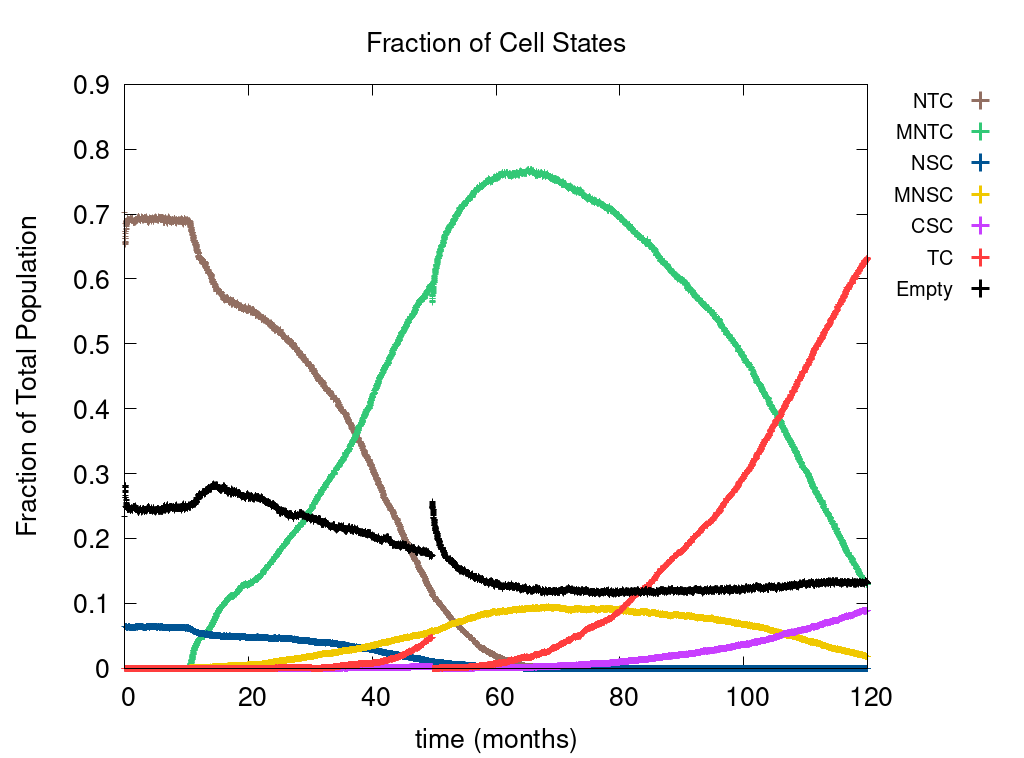
\includegraphics[width=\textwidth]{images/5_TumourExcisions/Fig1/numState_all_Keep.png}
      \caption{Remove only tumour cells, i.e., keeping the field}
      \label{fig:TumourExcision_numState_Keep}
    \end{subfigure}
    \begin{subfigure}[t]{.49\textwidth}
      \centering
      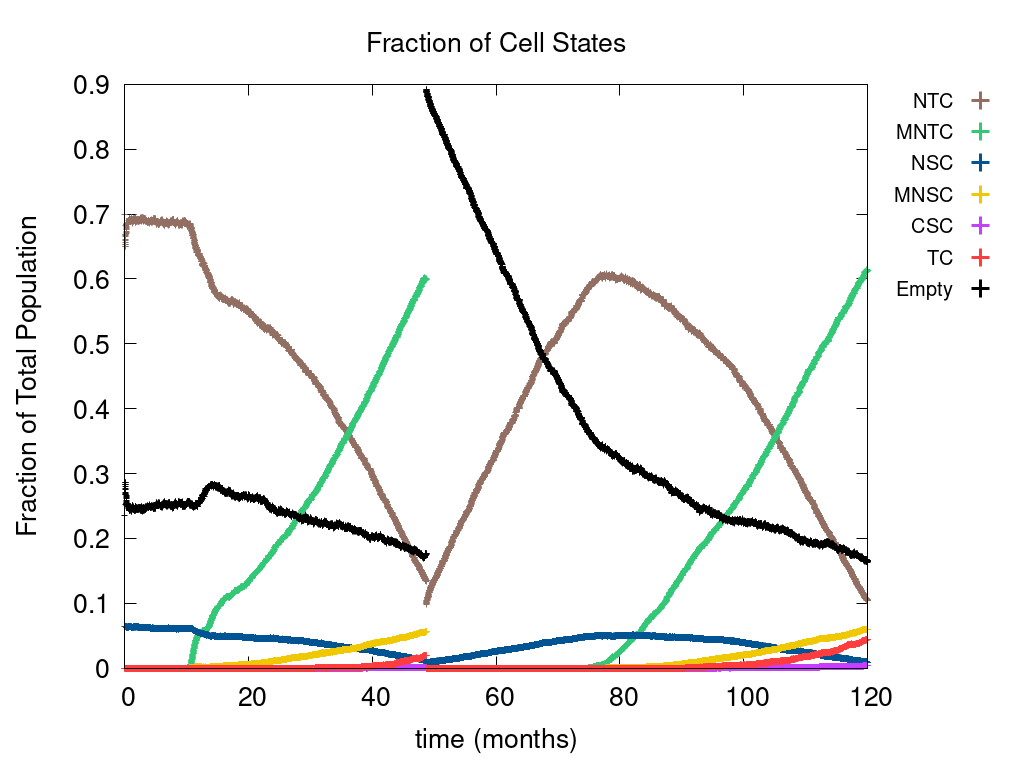
\includegraphics[width=\textwidth]{images/5_TumourExcisions/Fig1/numState_all_Remove.png}
      \caption{Remove all mutated cells, i.e., removing the field}
      \label{fig:TumourExcision_numState_Remove}
    \end{subfigure}
    \caption{In figures (a),(b) we show the time course of the fraction of cells in the different cell classes NTC, MNTC, NSC, MNSC, CSC, TC, empty. In the plots we consider the case where we (a) remove only TCs (keeping the field) and (b) we remove all mutated cells (removing the field). Parameters are as follows: grid size 256x256, both carcinogens activated, carcinogen spatial distribution 2, and time elapse of excision following first TC appearance was 18 months.}
    \label{fig:TumourExcision_numState}
\end{figure}

In Figure \ref{fig:TumourExcision_timeToRecur} we show the elapsed time it takes for cancer to recur after an excision has been performed some set amount of time after the first successful tumour cell(s) formed. In (a) we consider the case of keeping the field and in (b) we consider removing the field. Figure \ref{fig:TumourExcision_timeToRecur} in either case does not result with a linear graph due to the probabilistic nature of the CA model. In the case of keeping the field a linear downward trend is observed. This illustrates that the longer the elapsed time after the first TC forms and before excision, the less time it takes for the cancer to recur. This is to be expected because the remaining field will have developed more mutations over the course of time, is larger, and is more aggressive, which allows a tumour cell to recur faster. In the removing the field case there is no correlation between length of time before performing an excision and elapsed time before recurrence, there does, however, seem to be an upward trend, the values are in a similar range and can be attributed to random effects. Comparing keeping the field versus removing the field it is evident that it takes substantially longer for the cancer to recur in the case of removing the field.  
\begin{figure}[H]
    \centering
    \begin{subfigure}[t]{.49\textwidth}
      \centering
      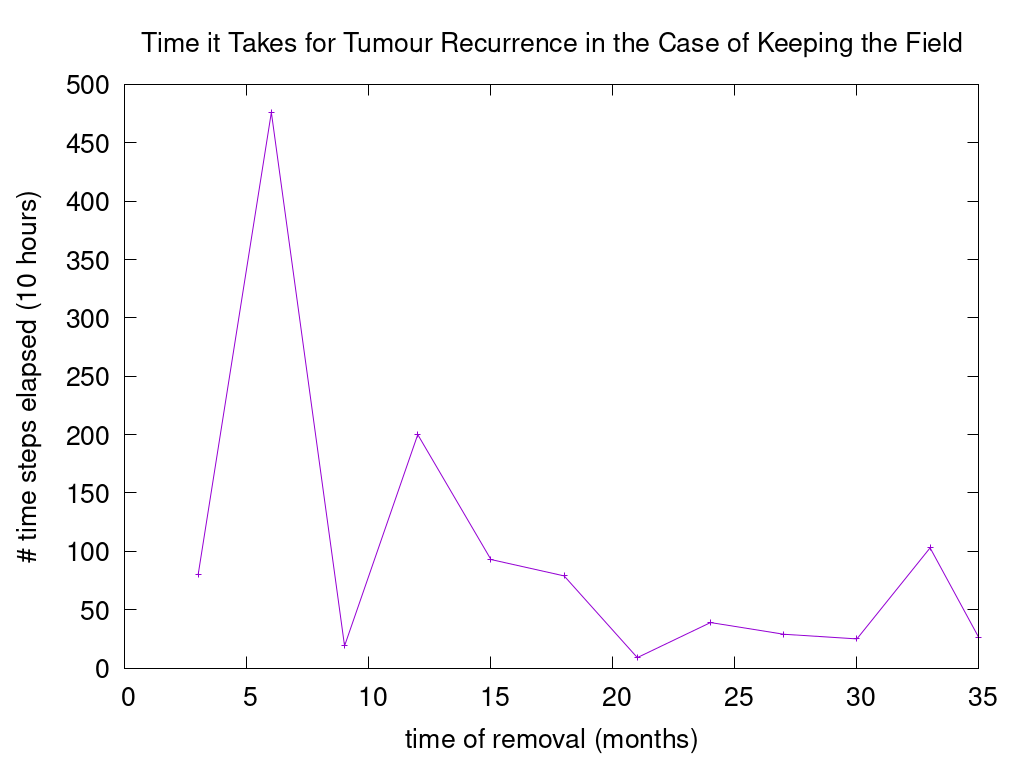
\includegraphics[width=\textwidth]{images/5_TumourExcisions/Fig2/timeToRecur_KeepField.png}
      \caption{Remove only tumour cells, i.e., keeping the field}
      \label{fig:TumourExcision_timeToRecur_Keep}
    \end{subfigure}
    \begin{subfigure}[t]{.49\textwidth}
      \centering
      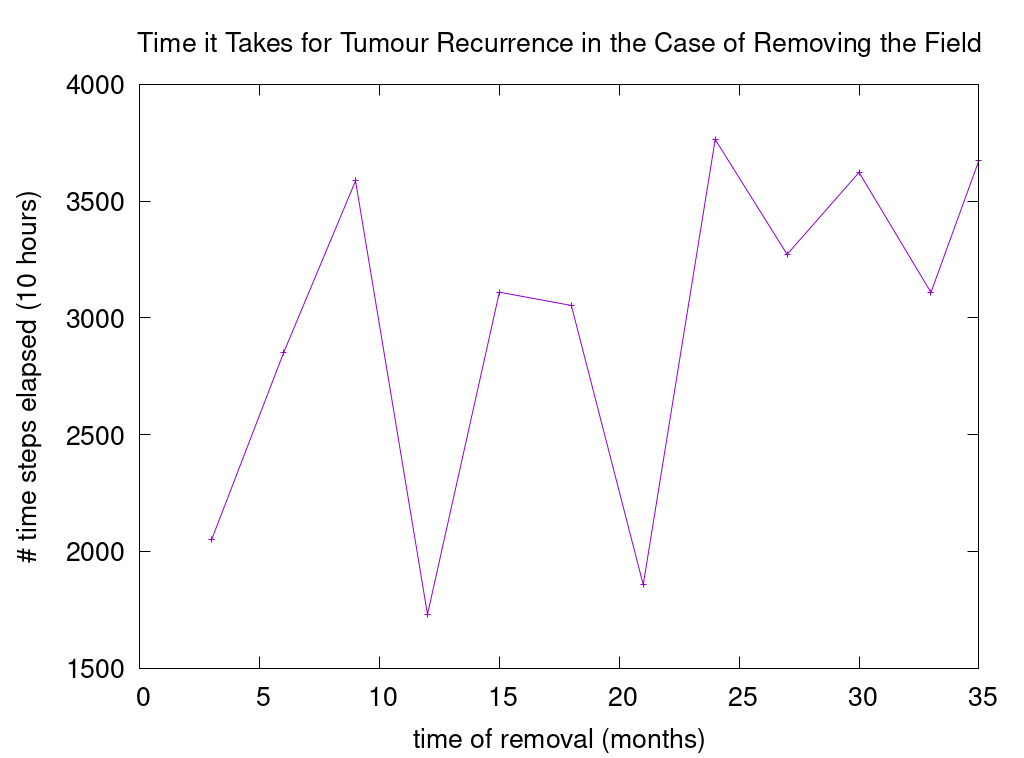
\includegraphics[width=\textwidth]{images/5_TumourExcisions/Fig2/timeToRecur_RemoveField.png}
      \caption{Remove all mutated cells, i.e., removing the field}
      \label{fig:TumourExcision_timeToRecur_Remove}
    \end{subfigure}
    \caption{In figures (a),(b) we show how long it takes for cancer to recur after excision has been completed on the tumour cells that were alive for a given number of months. In the plots we consider the case where (a) we remove only TCs (keeping the field) and (b) we remove all mutated cells (removing the field). Parameters are as follows: grid size 256x256, both carcinogens activated, carcinogen spatial distribution 2, and time elapse of excision following first TC appearance was 18 months.}
    \label{fig:TumourExcision_timeToRecur}
\end{figure}

If we were to include a wound healing mechanism in the model, the tissue would heal more rapidly and allow the first TC to recur faster, whether keeping the field or removing it. It is also important to note that in the case of keeping the field, if the domain at the time of excision is only made up of a large tumour mass, then all the cells will be killed off. Similarly, in the case of removing the field, if the field makes up the whole domain, then all the cells in the domain will be killed. These cases would be biologically realistic only in situations in which the excision removed the whole tumour mass and/or its surrounding field within a tissue or if the whole organ was removed. Recurrence would not happen at all if after the excision the individual was no longer exposed to the carcinogenic onslaught that originated the cancer field.

\end{document}